\documentclass[aspectratio=43]{beamer}
\usepackage[utf8]{inputenc}

%%%%%%%%%%%%%%%%%%%%%%%% THEME
\usetheme{material}
\useLightTheme
\usePrimaryBlueGrey
\useAccentDeepPurple

\usepackage{macros} % must come after theme

\title{High-Level Quantum Programming}
\keywords{\qk, \q Programming}

\begin{document}

\begin{frame}
	\titlepage
\end{frame}


\begin{frame}{Table of contents}
	\begin{card}
		\tableofcontents
	\end{card}
\end{frame}


\section{Introduction}
\begin{frame}{Meta-Introduction}
    \begin{card}
        By now, you should have a good grasp of the \textit{magic underneath the hood} of \qc. Meaning that quantum circuitry and quantum programming are now within your grasp.
    \end{card}
\pagenumber
\end{frame}

\begin{frame}{Introduction}
    \begin{cardTiny}
        This week, a different approach will be taken. We will see how quantum computing can be used for the benefit of many other scientific and industry areas. Hopefully, some of the topics you will learn will have a direct application on your life and work. 
    \end{cardTiny}
    \begin{cardTiny}
        We will do some \qka troubleshooting and then go through the latest examples on \href{https://github.com/Qiskit/qiskit-tutorial}{qiskit-tutorial} on how to use \qsa for solving real world problems. This example set is not fully explored and is expected to grow quite a lot in the short term (so keep your eyes open).\\
        \small{*If you are an autodidact, feel free to skip examples on areas that do not interest you.}
    \end{cardTiny}
\pagenumber
\end{frame}

\begin{frame}{Motivation}
    \begin{card}
    \begin{chapquote}[2pt]{\href{https://msramalho.github.io/}{Me}}
        ``The better people understand that quantum computing is within their grasp and can be leveraged towards personal gain, the sooner a day will come when running quantum algorithms is but a triviality.''
    \end{chapquote}
    \end{card}
\pagenumber
\end{frame}

\section{\qka}
\begin{frame}{\qka}
    \begin{center}
        
\includegraphics[width=1\textwidth]{qka}
    \end{center}
    \begin{card}
        As we saw in \href{\weekOne}{Week 1 - Quantum Tools}, \qka is the top-level block on the \qk full-stack infrastructure. This means it works on a higher level then what we have seen so far, abstracting a quantum compiler and providing an interface much similar to that of classical computing.
    \end{card}
\pagenumber
\end{frame}

\begin{frame}{The Premise of \qka}
    \begin{card}
        \qka contains ``a library of cross-domain quantum algorithms upon which applications for near-term quantum computing can be built''. \textbf{Near-term} means this is the time to look into this, as these algorithms and applications will become feasible in a short time. 
    \end{card}
\pagenumber
\end{frame}

\section{\q Supremacy}
\begin{frame}{\q Supremacy}
    \begin{card}
        The term \textbf{\q Supremacy} (not to be mistaken for a crossover between \textit{Quantum of Solace} and \textit{The Bourne Supremacy}...) stands for the moment in time in which quantum computers can do better than the most powerful computer in simulating a quantum system.\\
        This may seem strange, but the fact is that classical computers are so developed they they are still able to simulate better quantum computers than those in existence, but this classical "quantum simulation" fits into the \np family and so there will come a time, in the not so far away future, when they are no longer able to do better than \textit{the real thing}. 
    \end{card}
\pagenumber
\end{frame}

\begin{frameImg}[height]{quantum_supremacy.jpeg}

\end{frameImg}


\section{Running algorithms in \qka}
\begin{frame}{Running algorithms in \qka}
    \begin{card}
        First and foremost: \mintinline{bash}{pip install qiskit-aqua}
    \end{card}
    \begin{cardTiny}
        Then, we need to understand which algorithms have already been implemented in \qka. A comprehensive list can be found \href{https://qiskit.org/documentation/aqua/algorithms.html}{in the docs}, some that you may recognize are:
        \begin{itemize}
            \item \href{https://qiskit.org/documentation/aqua/algorithms.html#quantum-grover-search}{Grover Search}
            \item \href{https://qiskit.org/documentation/aqua/algorithms.html#quantum-dynamics}{Quantum Dynamics} (Simulating Universal Quantum Systems)
            \item \href{https://qiskit.org/documentation/aqua/algorithms.html#support-vector-machine-quantum-kernel-svm-q-kernel}{Support Vector Machine Quantum Kernel} (Machine Learning)
            \item \href{https://qiskit.org/documentation/aqua/algorithms.html#cplex}{CPLEX} (Constraint Solver)
        \end{itemize}
    \end{cardTiny}
\pagenumber
\end{frame}


\begin{frame}{Running algorithms in \qka}
\small{
    \qka is very declarative, in fact, running an algorithm can be thought of as defining a description of your problem, for instance in a \href{https://www.json.org/}{JSON} file or in a \href{https://docs.python.org/3/tutorial/datastructures.html#dictionaries}{Python Dictionary}. It is a composition of the following settings (For more information, check the \href{https://qiskit.org/documentation/aqua/execution.html#input-file}{docs}.):
    \begin{description}
        \item[Problem] The type of experiment (\mintinline{python}{"energy" | "excited_states" | "ising" | "search" ...})
        \item[Input/Oracle] The way to specify the input to the problem, depends on the type (SAT configuration, dataset, oracle, ...)
        \item[Algorithm] Optional specification of the algorithm to use (each problem has default algorithms) and its configurations
        \item[Backend] Which device to use (simulator, real device), highly customizable with number of shots (how many times should an experiment be repeated), activate compiler optimization, specify device noise parameters, ...
    \end{description}
}
\pagenumber
\end{frame}

\section{Troubleshooting \qka}
\begin{frame}{Troubleshooting \qka}
    \begin{card}
        After installing head to a command line and run  \mintinline{bash}{qiskit_aqua_ui}. If nothing happens, you should make sure you add your python \mintinline{bash}{bin} folder to the \href{https://docs.alfresco.com/4.2/tasks/fot-addpath.html}{system variable path}, it should be something like: \mintinline{python}{"C:/Program Files/Python36/Library/bin"}.\\
        The same solution goes for \href{https://stackoverflow.com/questions/14778178/import-cvxopt-base-the-specified-module-could-not-be-found}{the cvxopt error} when running python scripts.
    \end{card}
\pagenumber
\end{frame}

\begin{frame}{Troubleshooting \qka}
    \small{When everything is properly installed you should see something like (The \qka GUI for editing experimental settings):}
    \begin{center}
        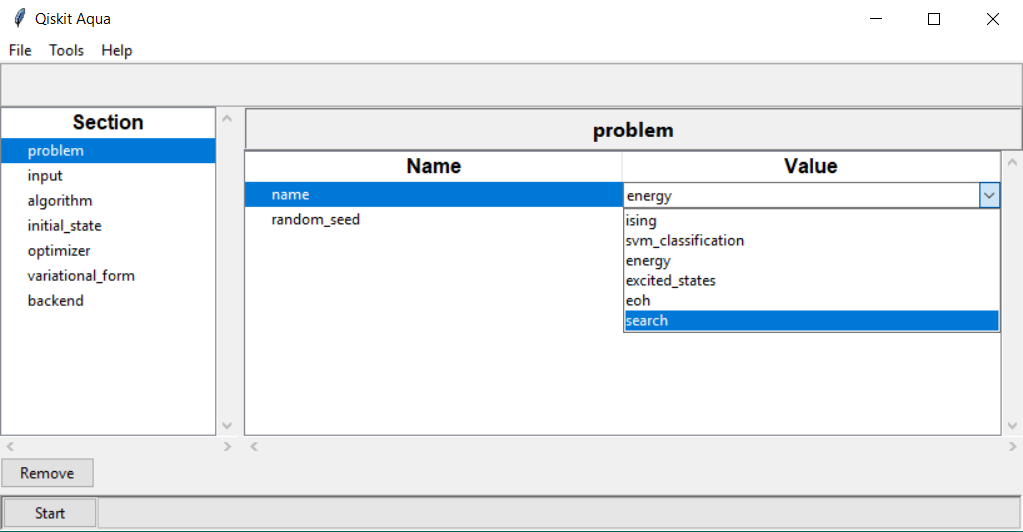
\includegraphics[width=1\textwidth]{qskit_aqua_ui}
    \end{center}
\pagenumber
\end{frame}

\section{\gvsa in \qka}
\begin{frame}[fragile]{\gvsa in \qka}
Go ahead and run the following code, while trying to understand it:\begin{minted}{python}
from qiskit_aqua import run_algorithm
# problem in DIMACS CNF format:
sat_cnf = """
p cnf 3 5
-1 -2 -3 0
1 -2 3 0
1 2 -3 0
1 -2 -3 0
-1 2 3 0
"""
params = {
    'problem': {'name': 'search'},
    'oracle': {'name': 'SAT', 'cnf': sat_cnf},
    'algorithm': {'name': 'Grover'},
    'backend': {'name': 'qasm_simulator'}
}
print(run_algorithm(params)['result']) # [1, -2, 3] or another
\end{minted}
\end{frame}



\section{\ai}
\begin{frame}{\ai}
\begin{card}
    If you work in Machine Learning, you probably know how the  \href{https://en.wikipedia.org/wiki/Support_vector_machine}{Support Vector Machine}(SVM) works. It is simply an algorithm for \href{https://en.wikipedia.org/wiki/Supervised_learning}{supervised learning}.\\
    \qka comes with more than one implementation of SVM Kernels. We will have a complete exercise on it this week (optional). 
\end{card}
\begin{card}
    More \ai related algorithms are expected to be implemented on \qka in the future, and you may even \href{https://qiskit.org/documentation/aqua/extending.html#algorithms}{implement your own}!
\end{card}
\pagenumber
\end{frame}

\begin{frame}[fragile]{\ai (SVM)}
\small{Here's an example of a configuration for an SVM classification model:}\begin{minted}{python}
params = {
    'problem': {
        'name': 'svm_classification',
        'random_seed': 1219 # same seed ensures reproducibility
    },
    'algorithm': {
        'name': 'QSVM.Kernel'
    },
    'backend': {
        'name': 'qasm_simulator',
        'shots': 1024
    },
    'feature_map': {
        'name': 'SecondOrderExpansion',
        'depth': 2,
        'entanglement': 'linear'
    }
}
\end{minted}
\end{frame}

\section{Optimization}
\begin{frame}{Optimization}
\begin{cardTiny}
    Still related to AI, there is another very important topic nowadays in both research and industry settings: \textbf{optimization}.
\end{cardTiny}
\begin{cardTiny}
    In this week's exercises you will have 2 examples of optimization problems: \href{https://en.wikipedia.org/wiki/Maximum_cut}{maximum cut} and the iconic \href{https://en.wikipedia.org/wiki/Travelling_salesman_problem}{traveling salesman problem}. These can both be reduced to a traditional model called \href{https://en.wikipedia.org/wiki/Ising_model}{ising model} that has been studied from a \href{https://arxiv.org/ftp/arxiv/papers/1210/1210.0113.pdf}{quantum point of view}. Thus, by using the ising solver in \qka we are able to solve many different problems, literally the only limitation is our ability to map problem formulations into know and solved problems.
\end{cardTiny}
\pagenumber
\end{frame}




\section{Chemistry in \qka}
\begin{frame}{Chemistry in \qka}
\begin{card}
    Lastly, and especially directed at chemistry related research, there are also examples of extrapolation of quantum mechanical properties that allow to make simulation on the behaviour of atoms, electrons and on the evolution of molecule configurations.\\ If you think about it, what better to simulate an atomic process than quantum?
\end{card}
\begin{card}
    As a matter of fact, there is a \href{https://github.com/Qiskit/aqua-chemistry}{complete repository} form the \qk team dedicated to chemistry algorithms for research on the field.
\end{card}
\pagenumber
\end{frame}

\begin{frame}[fragile]{Chemistry in \qka}
\small{We will not go much deeper into explaining the typical approaches, as this should be done by those students that truly benefit from it. However, here is an example of how such problems may be configured (the input comes from \href{https://support.hdfgroup.org/HDF5/whatishdf5.html}{HDF5} files):}\begin{minted}{python}
# Input dictionary to configure Qiskit aqua Chemistry
# for the chemistry problem.
aqua_chemistry_dict = {
    'driver': {'name': 'HDF5'},
    'HDF5': {'hdf5_input': 'H2/0.7_sto-3g.hdf5'},
    'operator': {'name': 'hamiltonian'},
    'algorithm': {'name': 'VQE'},
    'optimizer': {'name': 'COBYLA'},
    'variational_form': {'name': 'UCCSD'},
    'initial_state': {'name': 'HartreeFock'},
    'backend': {'name': 'statevector_simulator'}
}
\end{minted}
\end{frame}


\section{Hands-on}
\begin{frame}{Hands-on}
\begin{card}
    This week there will be quite a few exercise tutorials available, each student is expected to select and study at least one of them. Here are the topics covered in each:
    \begin{enumerate}
        \item Grover algorithm with \qka (search)
        \item SVM for Breast Cancer classification (\ai)
        \item Maximum Cut problem (optimization)
        \item Traveling Salesman problem (optimization)
        \item Computing the ground state energy of an $H_2$ molecule (Chemistry)
    \end{enumerate}
\end{card}
\end{frame}


\section{Where to learn more?}
\begin{frame}{Where to learn more?}
\begin{card}
    \begin{itemize}
        \item \href{https://qiskit.org/documentation/aqua/index.html}{\qka documentation} seriously a good point to start
        \item \href{https://github.com/Qiskit/qiskit-tutorial/tree/master/qiskit/aqua}{\qka official tutorials}
        \item \href{https://github.com/Qiskit/qiskit-tutorial/tree/master/community/aqua}{\qka community tutorials}
        \item \href{https://en.wikipedia.org/wiki/Quantum_programming}{A comprehensive analysis of \q Programming SDKs and languages} including, of course, \qk
    \end{itemize}
\end{card}
\end{frame}
\end{document}
